\documentclass[12pt,a4paper]{article}

\usepackage[margin=15mm]{geometry}
\usepackage{fontspec}
\setmainfont{GFS Artemisia}
\usepackage[greek, english]{babel}
\author{Κωνσταντίνος Χατζηαντωνίου 8941 \\ Εργασία 1}
\title{Ενσωματωμένα Συστήματα Πραγματικού Χρόνου}
\date{Μάιος 5, 2019}

\usepackage{hyperref} 
\usepackage{amsmath}
\usepackage{amsfonts}
\usepackage{amssymb}


\usepackage{xcolor}

\usepackage{graphicx}


\usepackage{tikz}
\usetikzlibrary{shapes,arrows}

\begin{document}

\maketitle

\section*{Εισαγωγή}

Στη εργασία αυτή υλοποιείται τακτική δειγματοληψία με προσπάθεια για μικρότερη δυνατή απόκλιση από τον πραγματικό χρόνο. Τα δείγματα αποτελούνται από τιμές της συνάρτησης  \textcolor{blue}{gettimeofday()}. Παρουσιάζονται 4 υλοποιήσεις: 2 χωρίς την χρήση των timestamps, με \textbf{interrupts} και με \textbf{sleep} και 2 με χρήση των timestamps με \textbf{sleep}.

\noindent
\textit{Code is available at:} \href{https://github.com/KonstantinosChatziantoniou/RealTimeEmbeddedSystems_Course}{\textcolor{blue}{github}}

\section{Χωρίς χρήση timestamps}

Υλοποιώντας την δειγματολήψία χωρίς την χρήση των timestamps, δεν έχουμε κανέναν έλεγχο στο διάστημα χρόνου μεταξύ διαδοχικών δειγμάτων. Αν υπάρξει κάποια καθυστέρηση, αυτή θα μετατοπίσει όλα τα δείγματα στον χρόνο και θα ξεπεράσουν τον συνολικό χρόνο που απαιτείται ή θα είναι λιγότερα.

\subsection{Interrupts-Alarm}
Για τη χρήση interrupts, αρχικά ρυθμίζουμε το διάστημα μεταξύ των interrupts και την συνάρτηση που θα καλείται με την \textcolor{blue}{settimer()}. Στην \textcolor{blue}{main} χρησιμοποιούμε την συνάρτηση \textcolor{blue}{pause()} για να μην καταναλώνεται ενέργεια μέχρι να σταματήσει η χρήση του timer.

Όταν καλείται η συνάρτηση σε κάθε interrupt αποθηκεύουμε την τιμή της  \textcolor{blue}{gettimeofday()} σε έναν πίνακα. Όταν φτάσουμε στον επιθυμητό αριθμό δειγμάτων, η συνάρτηση σταματάει τον timer και το πρόγραμμα αποθηκεύει τα αποτελέσματα και τελειώνει.

\subsubsection*{Στατιστικά}

\begin{itemize}
\item mean: 99999.995
\item median: 100000
\item min: 99391
\item max: 100786
\item standard deviation: 236.131
\end{itemize}

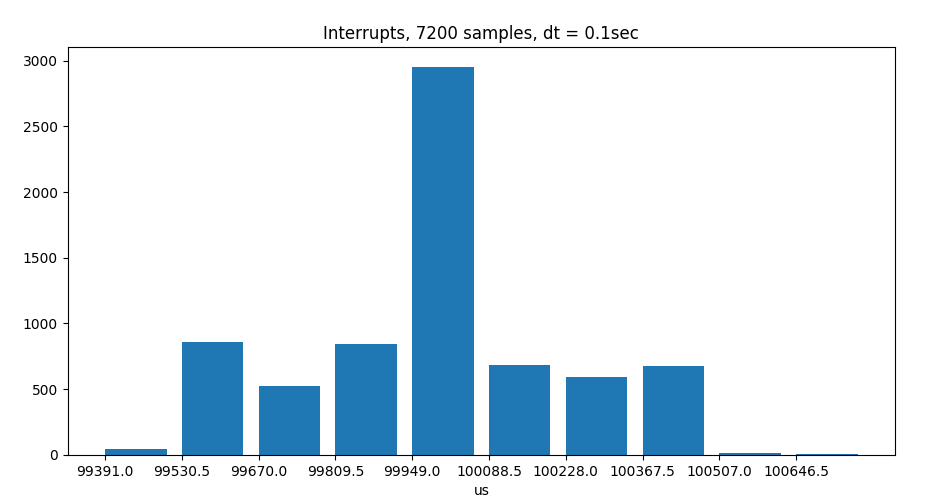
\includegraphics[scale=0.55]{intr_hist}

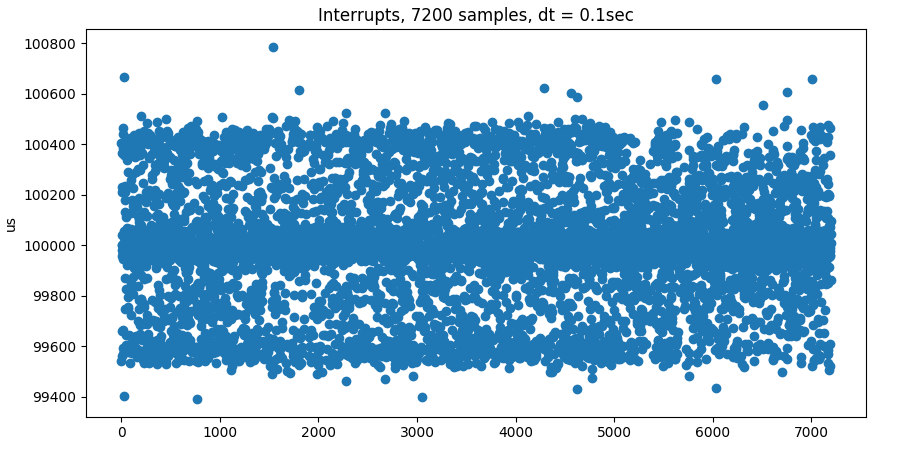
\includegraphics[scale=0.55]{intr_sctr}


\subsection{Sleep}

H sleep χρησιμοποιείται μέσα σε ένα for loop στη main, για να σταματάει τον πρόγραμμα ανάμεσα στα δείγματα.


\subsubsection*{Στατιστικά}

\begin{itemize}
\item mean: 100367.268
\item median: 100451
\item min: 100042
\item max: 101000
\item standard deviation:  204.779
\end{itemize}


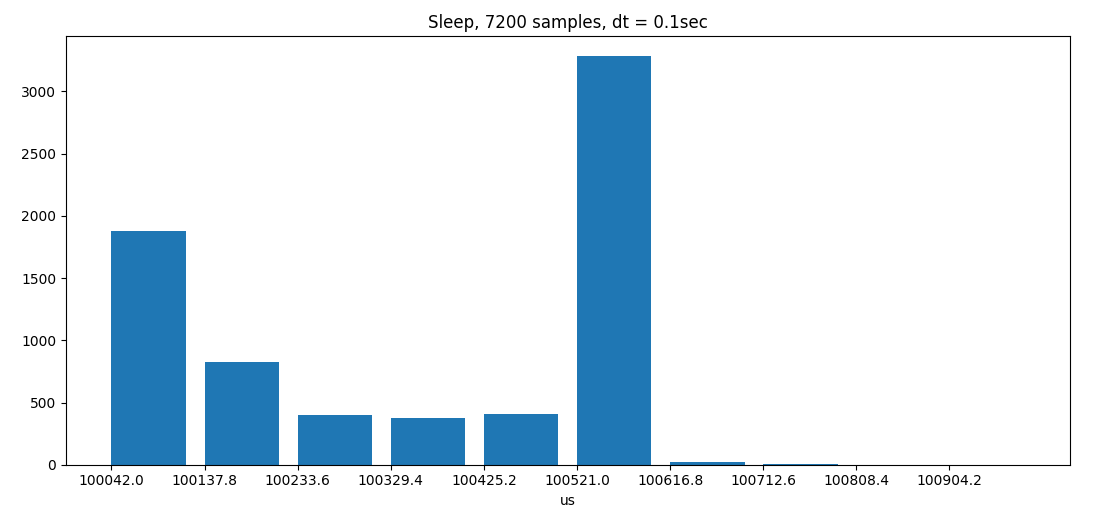
\includegraphics[scale=0.55]{sleep_hist}

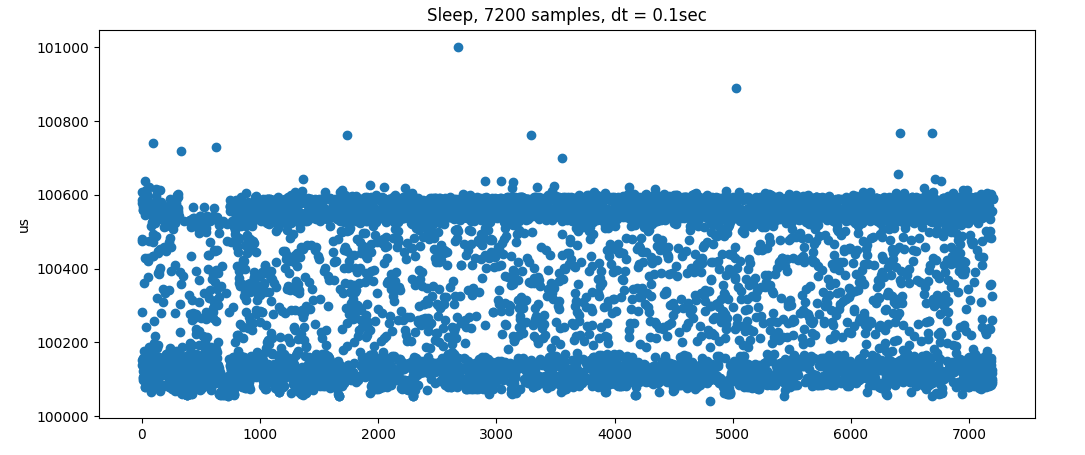
\includegraphics[scale=0.55]{sleep_sctr}


\section{Με χρήση timestamps}

\subsection*{Version 1}
Σε αυτήν την υλοποίηση, χρησιμοποιείται πάλι η συνάρτηση \textcolor{blue}{usleep()}, με την διαφορά ότι η χρόνος αναμονής είναι μεταβλητός.
Αρχικά ο χρόνος αναμονής dt, αλλάζει κατά $\pm$offset, ανάλογα άν καθυστέρησε ή ήρθε νωρίτερα το προηγούμενο δείγμα. Σημαντική λεποτμέρια είναι ότι πρέπει να λάβουμε υπόψην μας και το προηγούμενο offset όταν υπολογίζουμε το interval μεταξύ των προηγούμενων τιμών. Αν δεν το κάνουμε αύτο τα δείγματα θα απκλίνουν(ο μέσος όρος όμως θα παραμένει σωστός).


\subsubsection*{Στατιστικά}

\begin{itemize}
\item mean: 100000.011
\item median: 100000
\item min: 97070
\item max: 102917
\item standard deviation:  157.297
\end{itemize}

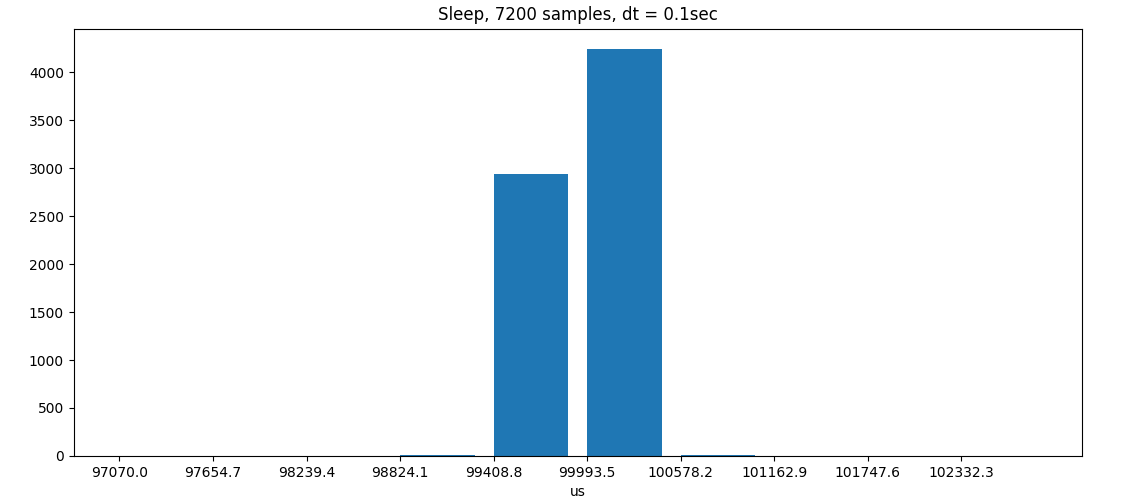
\includegraphics[scale=0.5]{cal_sleep_1_hist.png}

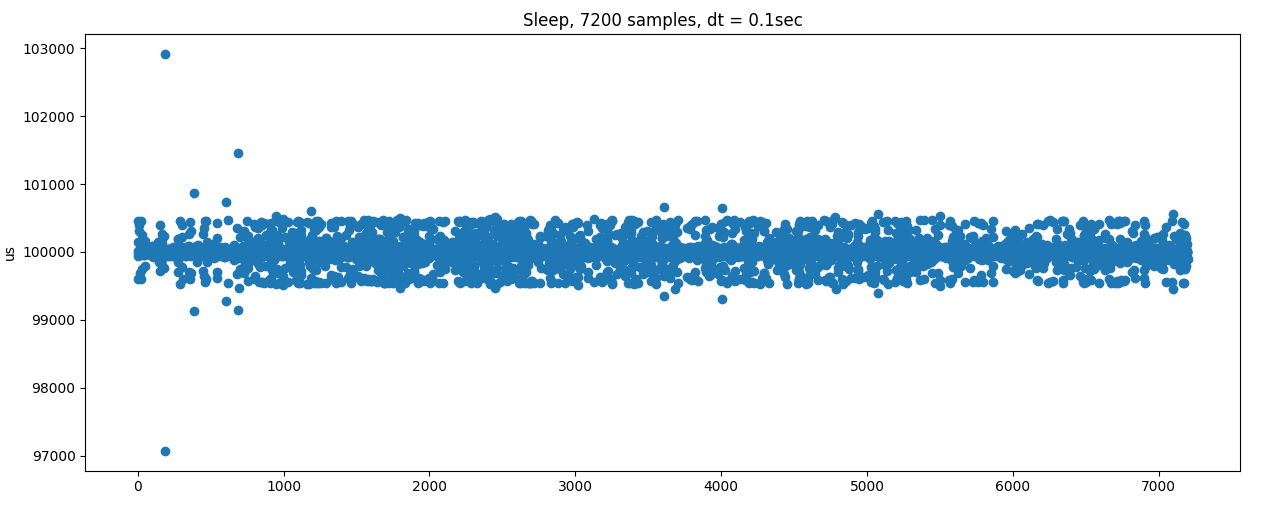
\includegraphics[scale=0.5]{cal_sleep_1_sctr.png}

Mε zoom:

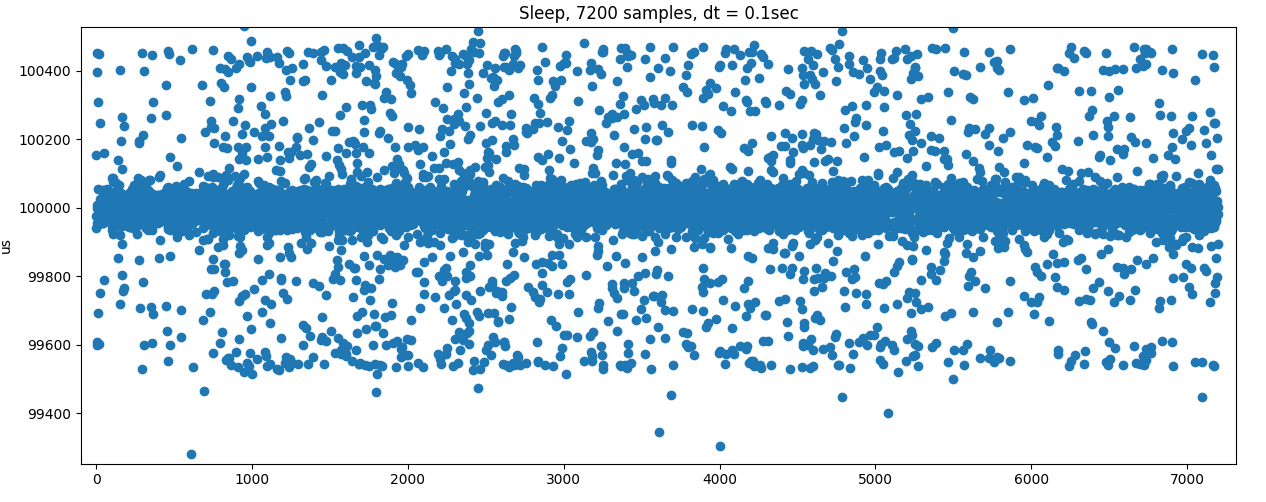
\includegraphics[scale=0.5]{cal_sleep_1_sctr_zoom.png}


Όλες οι τιμές βρίσκονται στο διάστημα [98824.1, 101747.6] εκτός από το μέγιστο και το ελάχιστο. Στο επόμενο σετ στατιστικών παραθέτονται τα καλύτερα αποτελέσματα που επιτεύχθηκαν, αλλά κατα παραπάνω είναι πιο αντιπροσωπευτικά του μέσου όρου πειραμάτων


\begin{itemize}
\item mean: 100000.010
\item median: 100000
\item min: 98301
\item max: 101680
\item standard deviation:  53.899
\end{itemize}

Πάλι όλα τα δείγματα βρίσκονται σε μικρότερο διάστημα ( [99314.7,100666.3,] ) εκτός από το μέγιστο και το ελάχιστο.


Mε zoom:

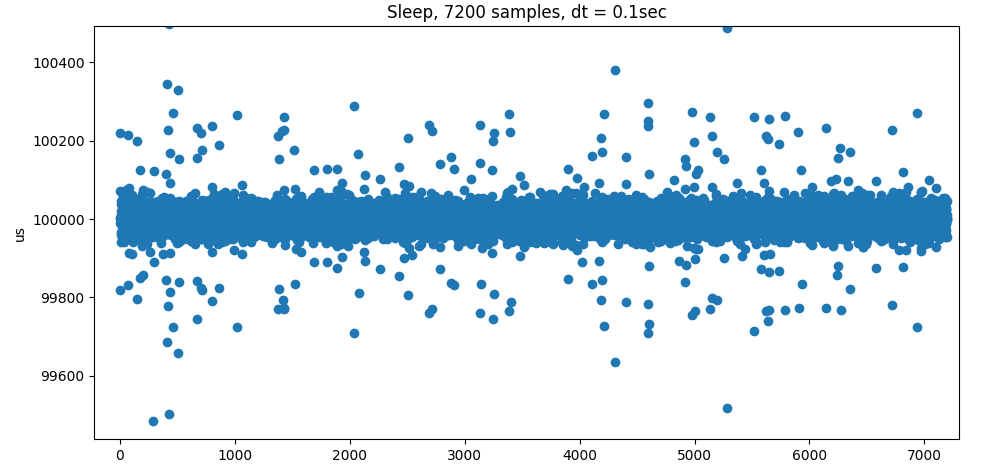
\includegraphics[scale=0.6]{cal_sleep_better_sctr_zoom.png}


\subsection*{Version 2}
Στη δεύτερη υλοποίηση της sleep με μεταβλητό χρόνο μεταβολής, αντί να μεταβάλουμε τον χρόνο αναμονής κατά offset = dt - actualTime, θα τον μεταβάλουμε κατά offset/2. Κίνητρο για αυτό είναι να μειώσουμε την επίδραση κάποιας ακραίας τιμής, η οποία θα προκαλέσει ακραία τιμή προς την αντίθετη κατεύθυνση για άμεση εξισορρόπηση της μέσης τιμής.

\begin{itemize}
\item mean: 100078.070
\item median: 100047
\item min: 99652
\item max: 100807
\item standard deviation:  145.753
\end{itemize}


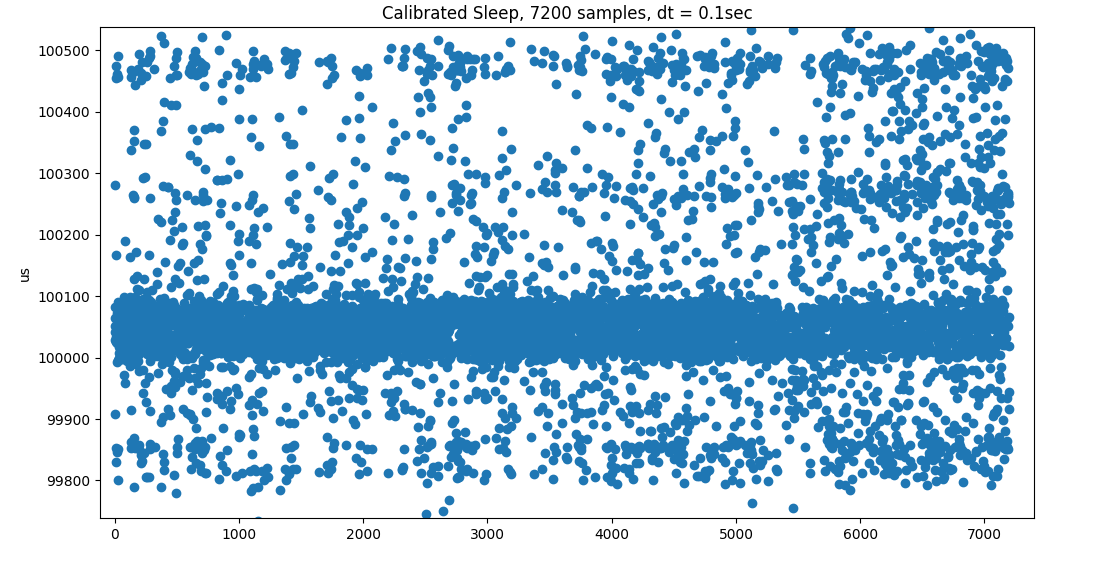
\includegraphics[scale=0.6]{cal_sleep_2_sctr.png}

Παρατηρούμε μικρή βελτίωση της τυπικής απόκλισης, καλή βελτίωση της min και max  τιμής,  αλλά χειρότερο μέσο όρο.


\section{Σύγκριση χρήσης/ μη χρήσης timestamps}

Όπως βλέπουμε, η συνάρτηση sleep() αποτυγχάνει να κρατήσει τον μέσο όρο κοντά στην επιθυμητή τιμή, λόγω εσωτερικής καθυστέρησης του συστήματος. Όμως έχει πολύ καλη τυπική απόκλιση. Θα μπορούσαμε να προσαρμώσουμε το dt κατά mean-dt αλλά δε μπορούμε να είμαστε βέβαιοι ότι θα δουλέυει πάντα σωστά, οπότε απορρίπτεται

Η χρήση timer και interrupts ήταν εύκολη και έφερε πολύ καλά αποτελέσματα. Φαίνεται ότι η timer εσωτερικά κρατάει τον μέσο όρο intervals στην επιθυμητή τιμή. Είχε καλή διακύμανση και το εύρος των τιμών ήταν 709+786.

Το version 1 πετυχαίνει εξίσου καλό μέσο όρο με τoν timer, αλλά πετυχαίνει καλύτερη τυπική απόκλιση. Το μέγιστο και το ελάχιστο είναι αρκετά πιο μακριά βέβαια, αλλά είναι μεμονωμένες περιπτώσεις.


Με το version 2 μπορούμε να μειώσουμε τα μεγάλα min max και την τυπική απόκλιση σε βάρος όμως του μέσου όρου(που μπορεί να μην είναι αποδεκτό)


Εν τέλει το version 1 του sleep με χρήση timestamps φαίνεται να είναι καλύτερο, εκτός αν για κάποιο λόγο οι μέγιστη/ελάχιστη τιμή είναι απογερυτικά μακριά για συγκεκριμένο συστημα.

\section{Χρήση CPU}

Σύμφωνα με τις ενδείξεις τις \textcolor{blue}{htop} με interval 0.05 sec, η χρήση CPU ήταν $0.00\%$.  Ο χρόνος χρήσης CPU για τις 2 πρώτες υλοποιήσεις χωρίς χρήση timestamps ήταν 0.15sec. Για τις επόμενες υλοποιήσεις ήταν 0.38 sec. Οι δύο αυτές τιμές είναι κατά πολύ μικρότερες από το συνολικό χρόνο εκτέλεσης (720 sec). 
Μπορούμε να πούμε ότι η κατανάλωση ενέργειας της διαδικασίας συλλογής δειγμάτων είναι αμελητέα, όπως και η διαφορά με το να χρησιμοποιούμε τα timestamps (μαζί με τη διαδικασία επεξεργασίας τους).

Η υλοποίηση με sleep και timestamps ,version 1, είναι καλύτερη από αυτή με interrupts, και αν δεν είναι πάρα πολύ αυστηρές οι απαιτήσεις σε ενέργεια συμφέρει να την χρησιμοποιήσουμε.

\end{document}